\documentclass[aspectratio=1610]{beamer}

\usepackage[utf8]{inputenc}
\usepackage{graphicx}
\usepackage{amssymb}
\usepackage[export]{adjustbox}
\usetheme{Frankfurt}
\usefonttheme[onlymath]{serif}
\usepackage[super]{nth}
\graphicspath{{./Figure/}}
\usepackage{hyperref}
\usepackage{listings}
\hypersetup{
    colorlinks=true,
    linkcolor=blue,
    filecolor=magenta,      
    urlcolor=cyan,
}
\definecolor{satinsheengold}{rgb}{0.85, 0.63, 0.21}
\setbeamercolor{structure}{fg=satinsheengold}
\setbeamercolor{title}{fg=black}
\setbeamercolor{title in head/foot}{fg=black, bg=satinsheengold}
\setbeamercolor{author}{fg=black}
\setbeamercolor{frametitle}{fg=black}
\setbeamercolor{author in head/foot}{fg=black, bg=satinsheengold}
\setbeamercolor{institute in head/foot}{bg=satinsheengold}
\setbeamercolor{date in head/foot}{bg=satinsheengold}
\setbeamercolor{navigation symbols}{fg=gray}
\setbeamercolor{block title}{bg=black}
\setbeamercolor{item projected}{fg=black}
\setbeamertemplate{blocks}[rounded][shadow=false]
\setbeamertemplate{enumerate items}[circle]
%\setbeamertemplate{footline}[frame number]
%Adding frame #s
\setbeamertemplate{navigation symbols}{%
    \usebeamerfont{footline}%
    \usebeamercolor[fg]{footline}%
    \hspace{1em}%
    \insertframenumber/\inserttotalframenumber
}

\title{Coding Assignment 1 Write-up}
\author{Andrew Sivaprakasam}

\date{03/20/2021}


\begin{document}
\frame{\titlepage}

\begin{frame}
\frametitle{Question 2$|$ One-Way Sensitivity Analysis Tornado Plots}
\small{Observations of how sensitive the model output is to the specified parameters. }
\begin{center}
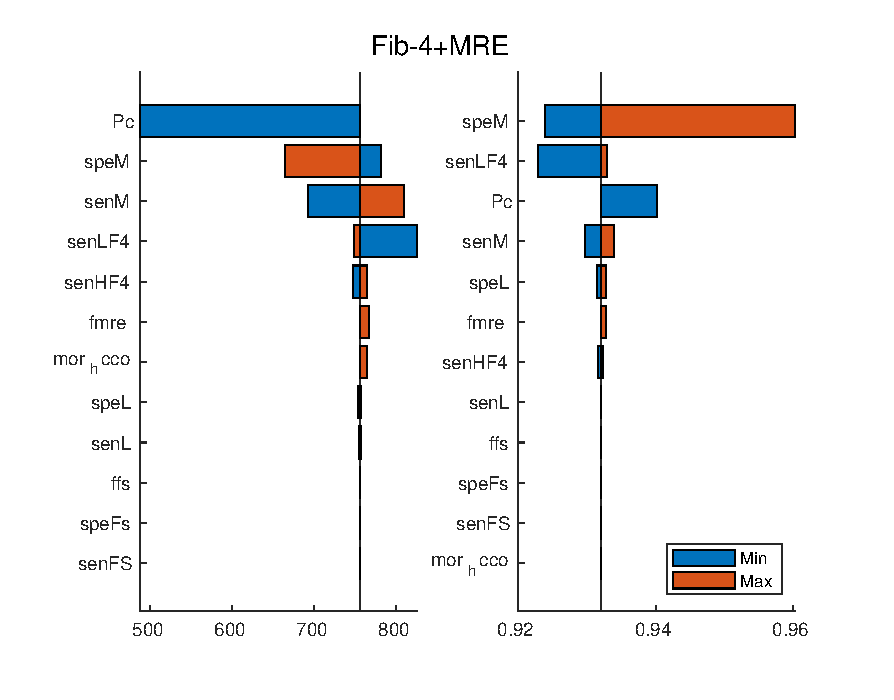
\includegraphics[width = .36\textwidth]{sens1}
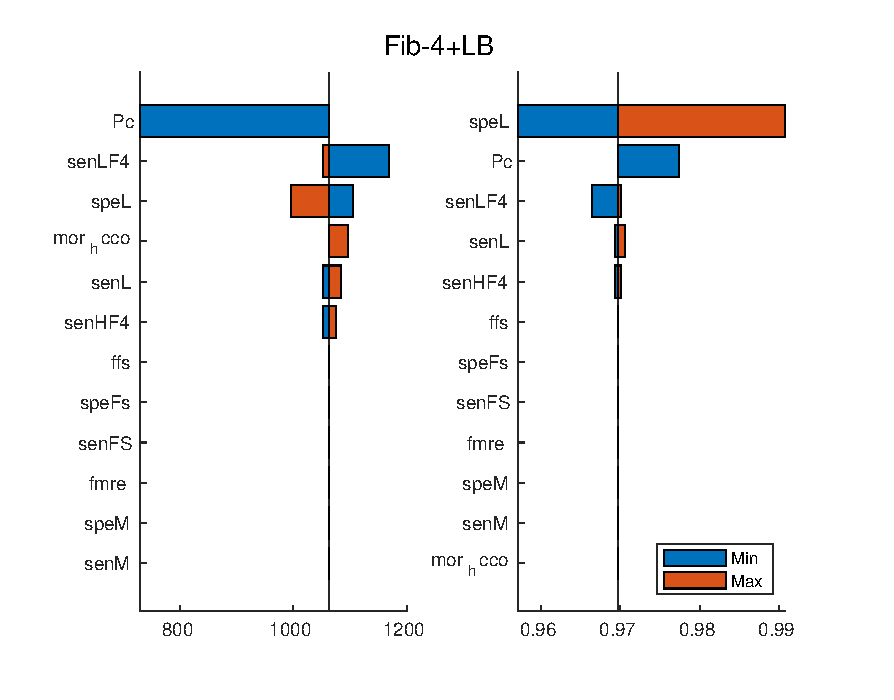
\includegraphics[width = .36\textwidth]{sens2}
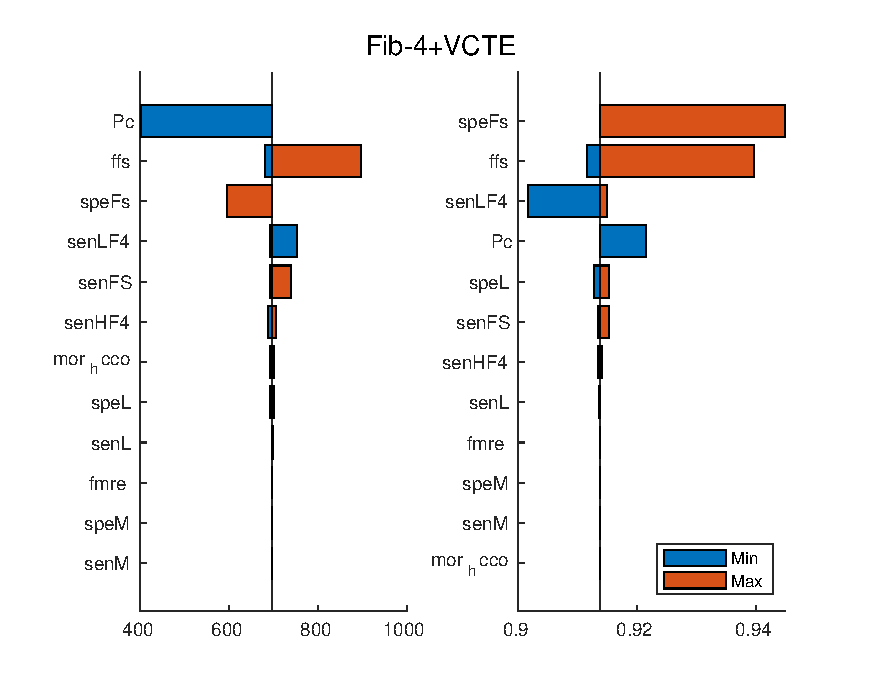
\includegraphics[width = .36\textwidth]{sens3}
\end{center}
\end{frame}

\begin{frame}
\frametitle{Question 3a$|$ Full-Factorial Histograms}

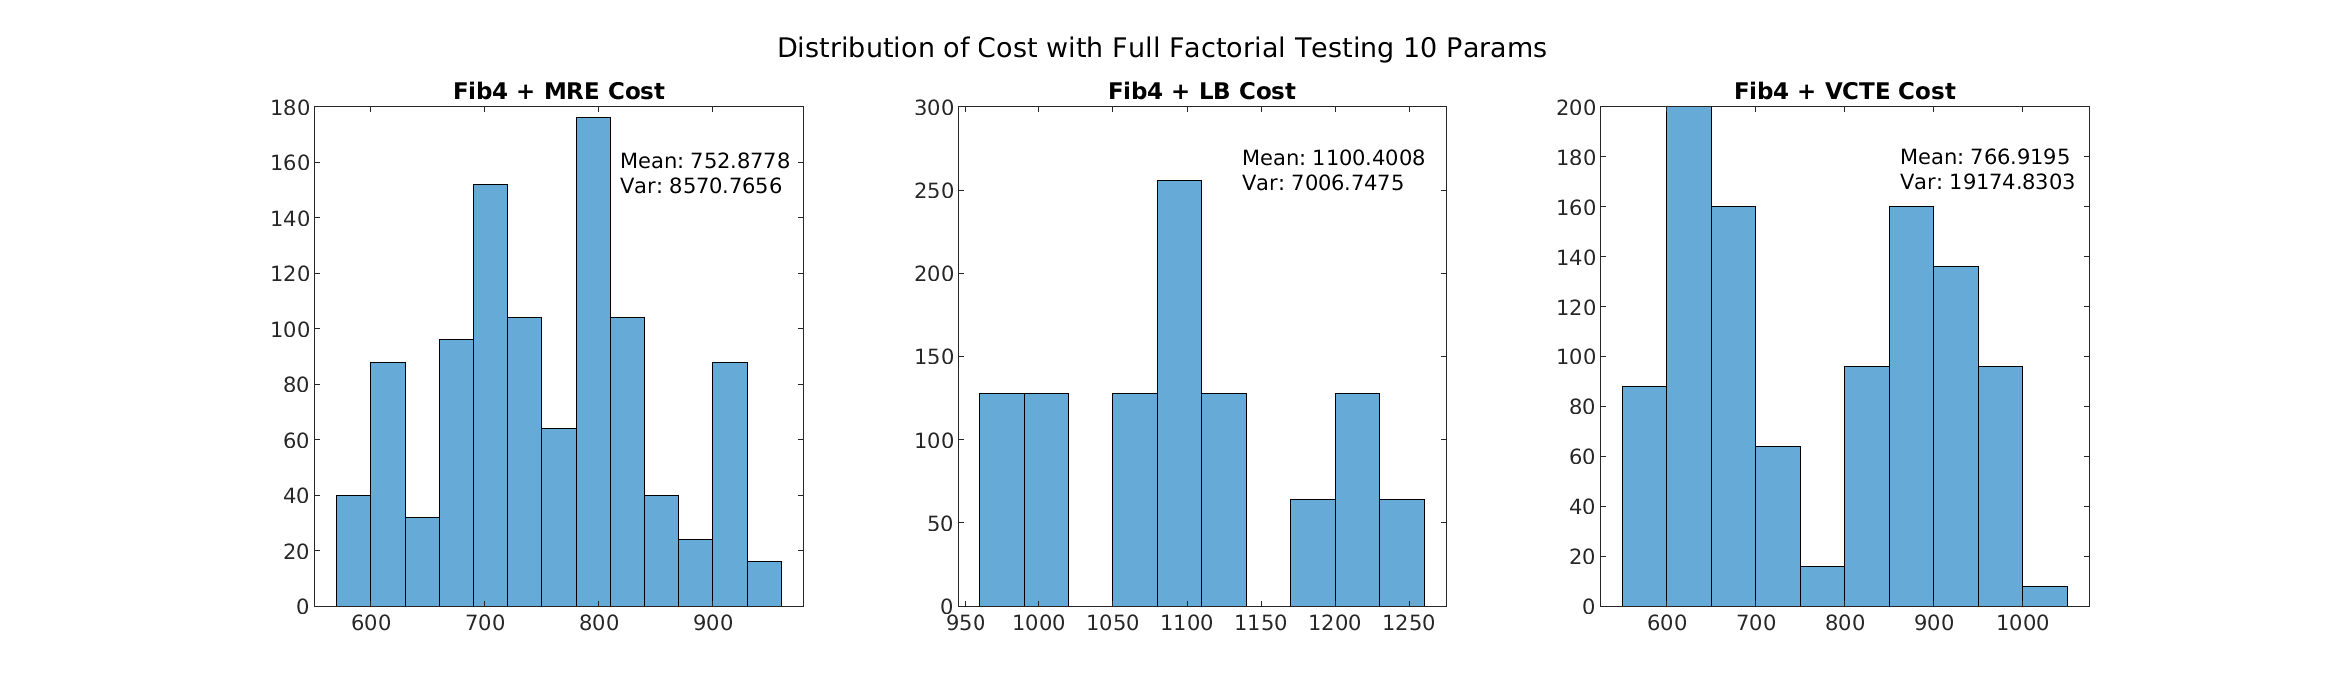
\includegraphics[width = \textwidth]{cost_distributions}
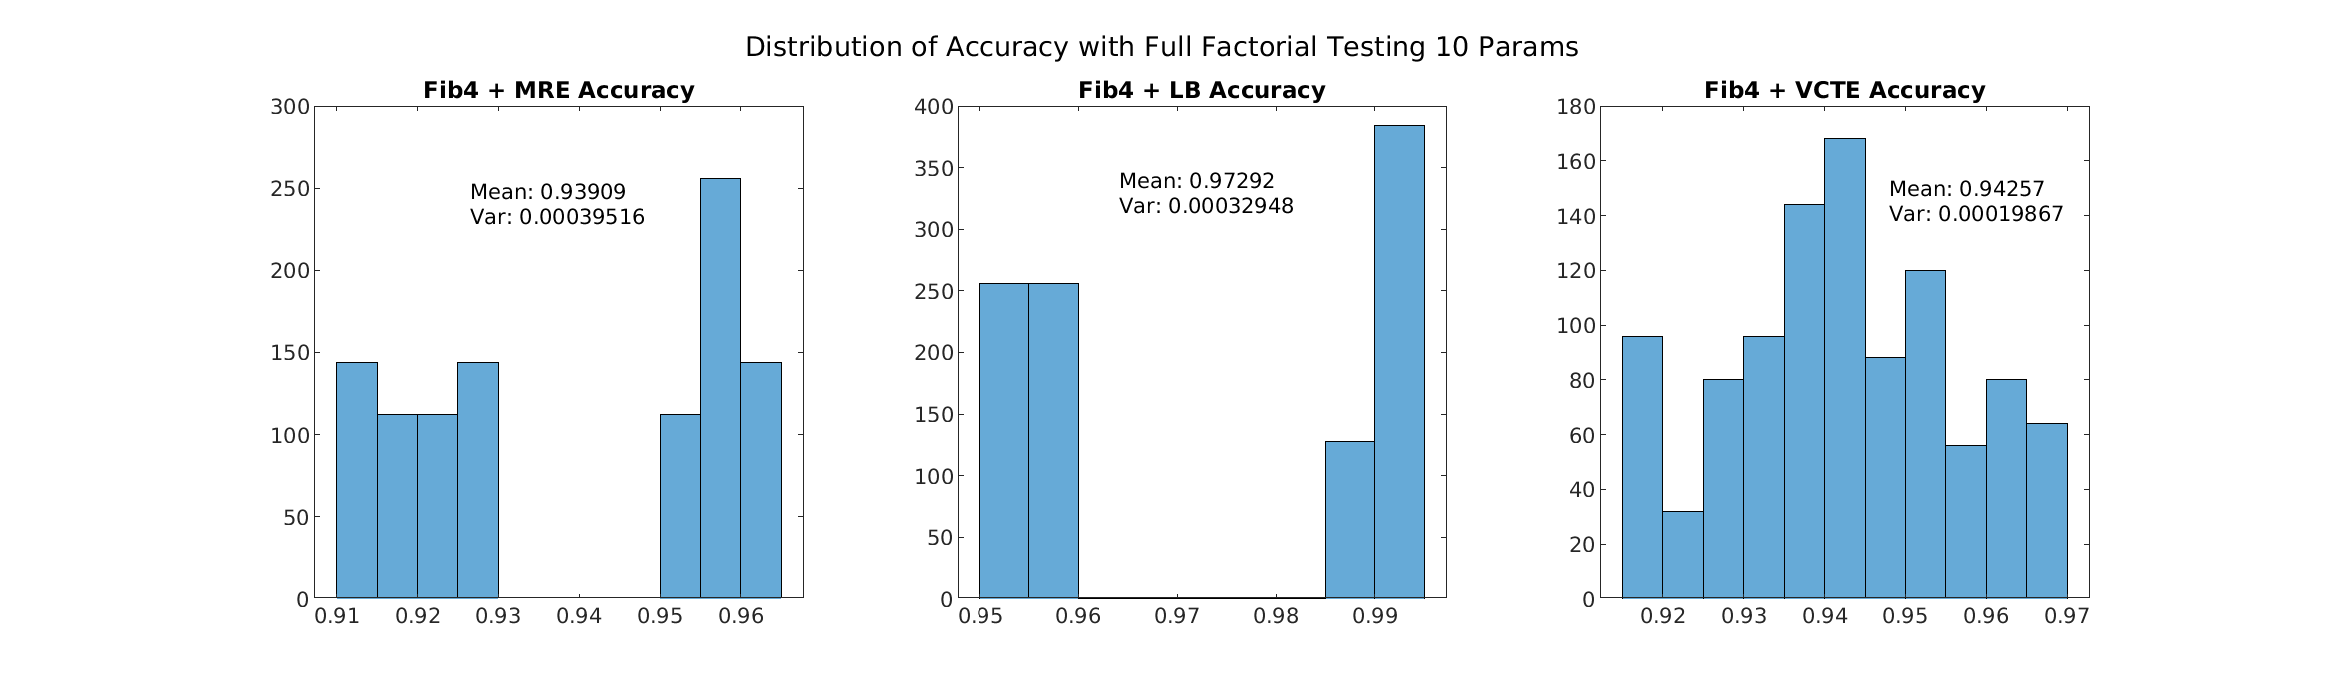
\includegraphics[width = \textwidth]{accuracy_distributions}

\end{frame}

\begin{frame}
\frametitle{Question 3a$|$ Full-Factorial Fitted Distributions}
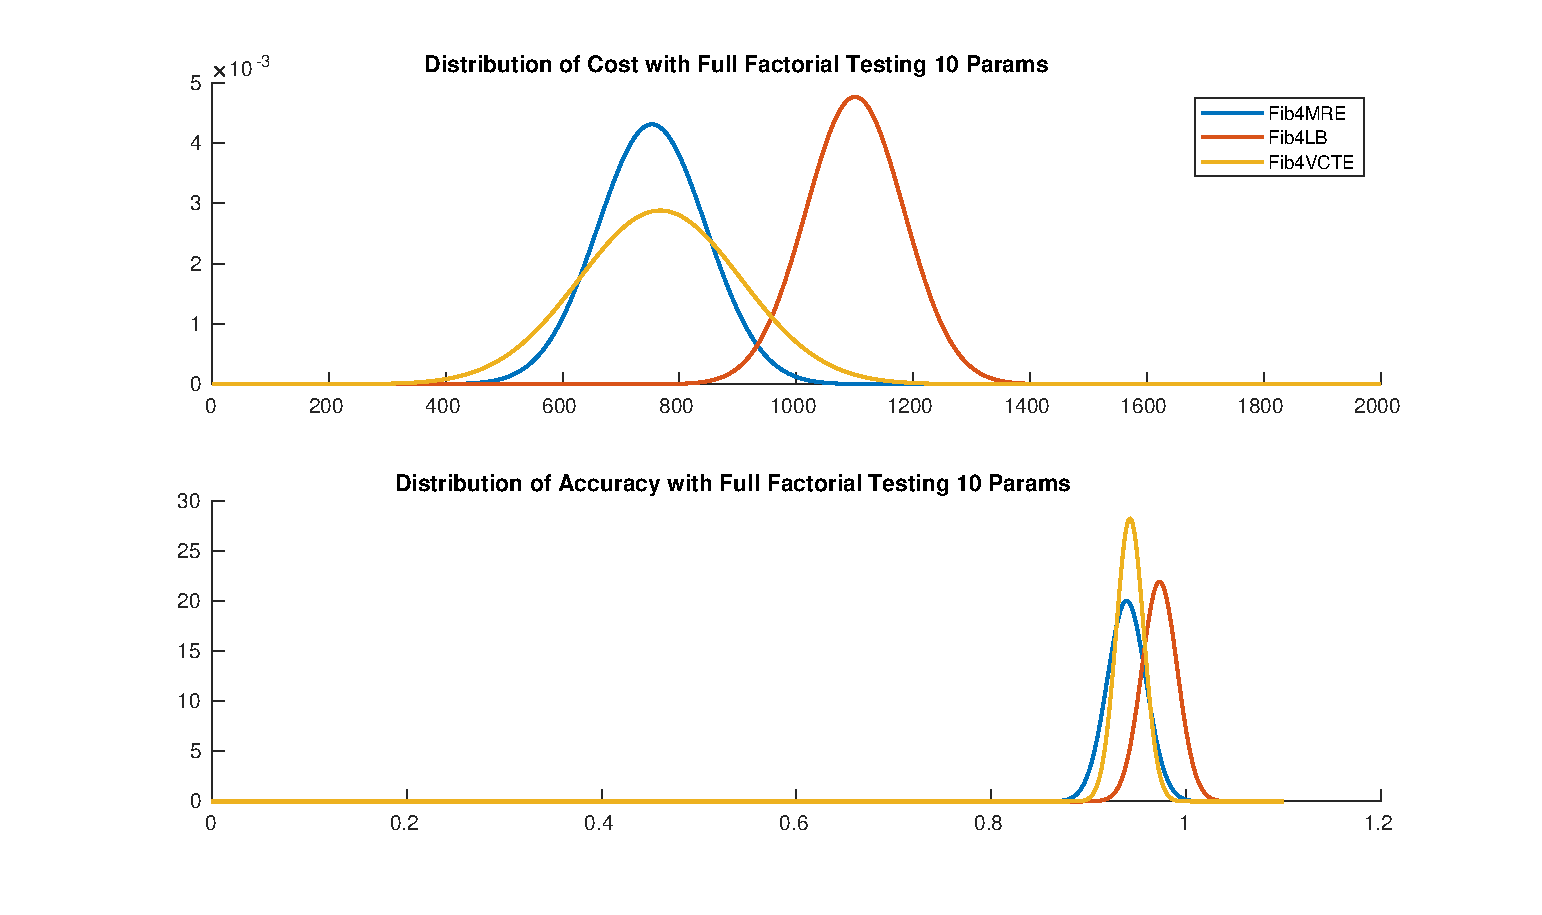
\includegraphics[width = \textwidth]{fitted_dist}
\end{frame}

\begin{frame}[fragile]
\frametitle{Question 3b$|$ Full-Factorial Percent > 300 (from Code)}
The percent of trials where the difference $|LB_{cost} - MRE_{cost}| > 300$ was \underline{61.7188}\%

\vspace{2em}
See \verb|q3.m|  252-253:

\begin{center}
\begin{verbatim}
diff = abs(Fib4MRE_cost_out-Fib4LB_cost_out);
percent_greater = sum(diff>300)*100/L;
\end{verbatim}
\end{center}
\end{frame}

\begin{frame}[fragile]
\frametitle{Question 3c$|$ Full-Factorial Sensitivity Analysis on \underline{MRE}}

The effect of varying MRE specificity and sensitivity params ( \verb|speM| \& \verb|senM| ) on the cost difference between MRE and LB can be visualized as follows:
\vspace{1.5em}

\centering
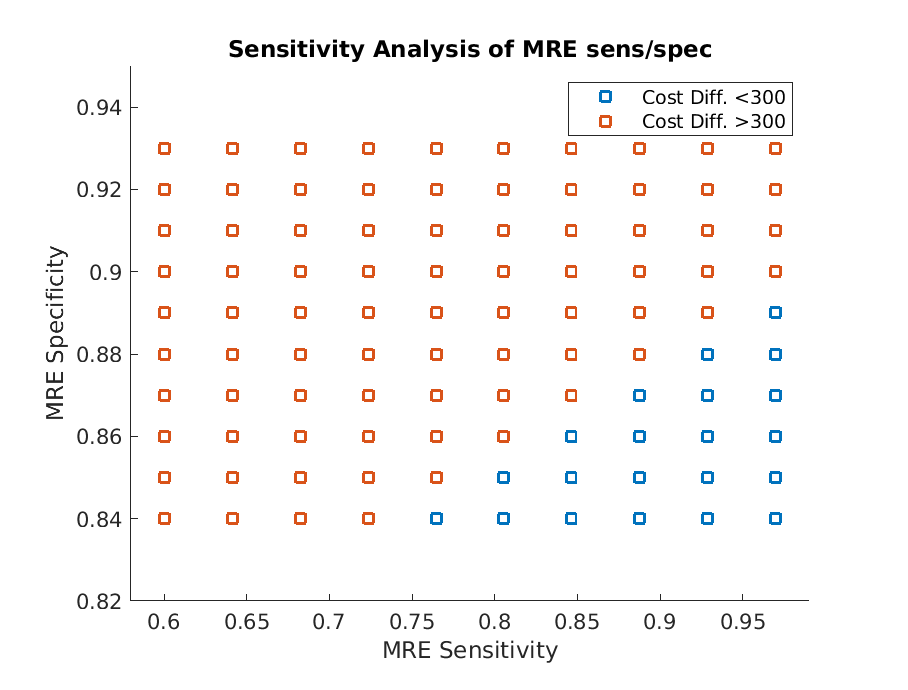
\includegraphics[width = .49\textwidth]{3c_1}
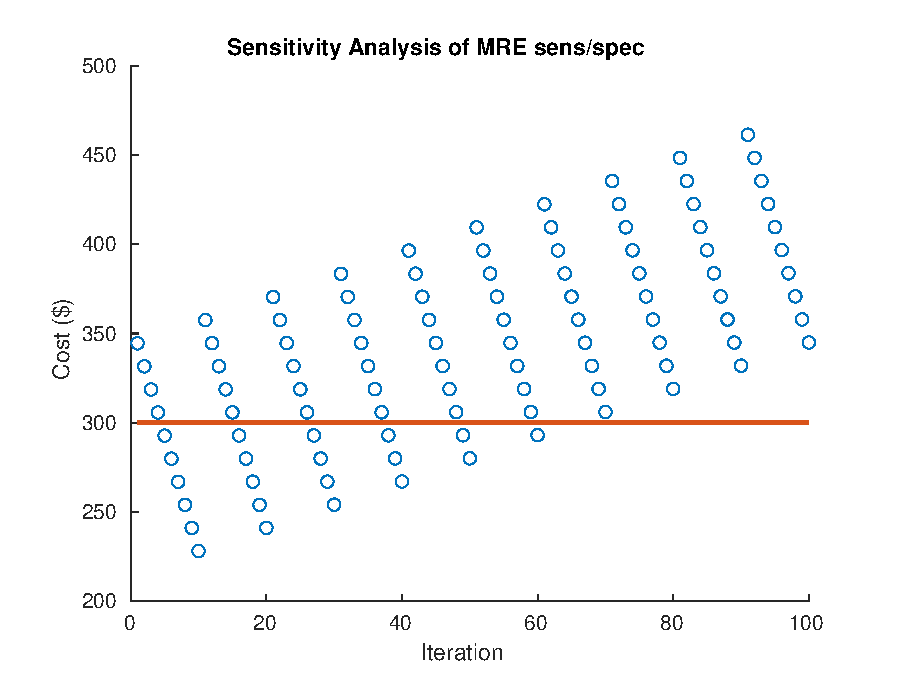
\includegraphics[width = .49\textwidth]{3c_2}

\textit{\underline{79\%} of the simulated outputs for cost difference were greater than 300.}

\end{frame}

\begin{frame}[fragile]
\frametitle{Question 3d$|$ Full-Factorial Sensitivity Analysis on \underline{LB}}

The effect of varying LB specificity and sensitivity params ( \verb|speM| \& \verb|senM| ) on the cost difference between MRE and LB can be visualized as follows:
\vspace{1.5em}

\centering
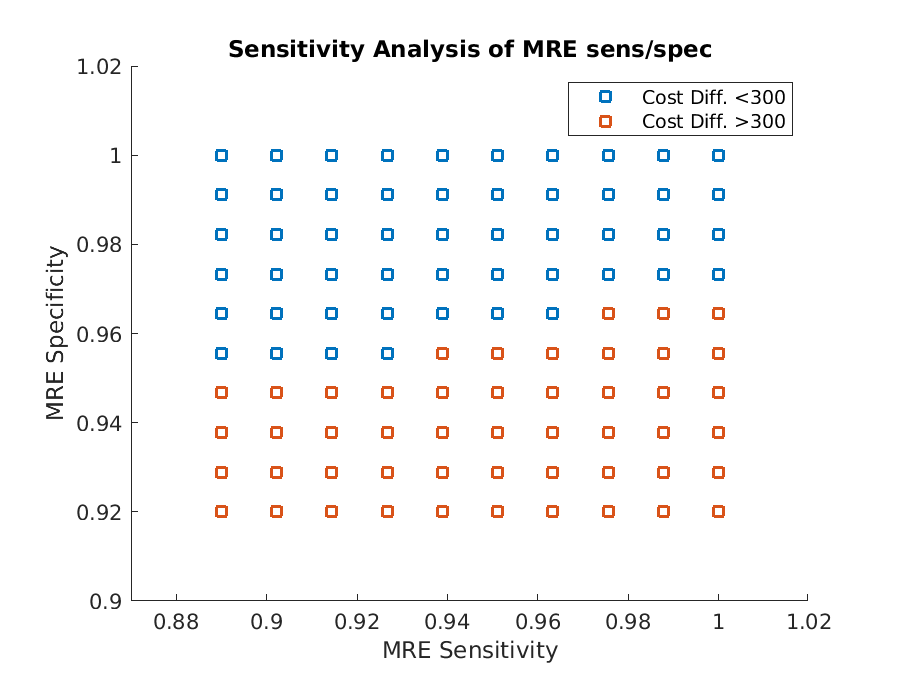
\includegraphics[width = .49\textwidth]{3d_1}
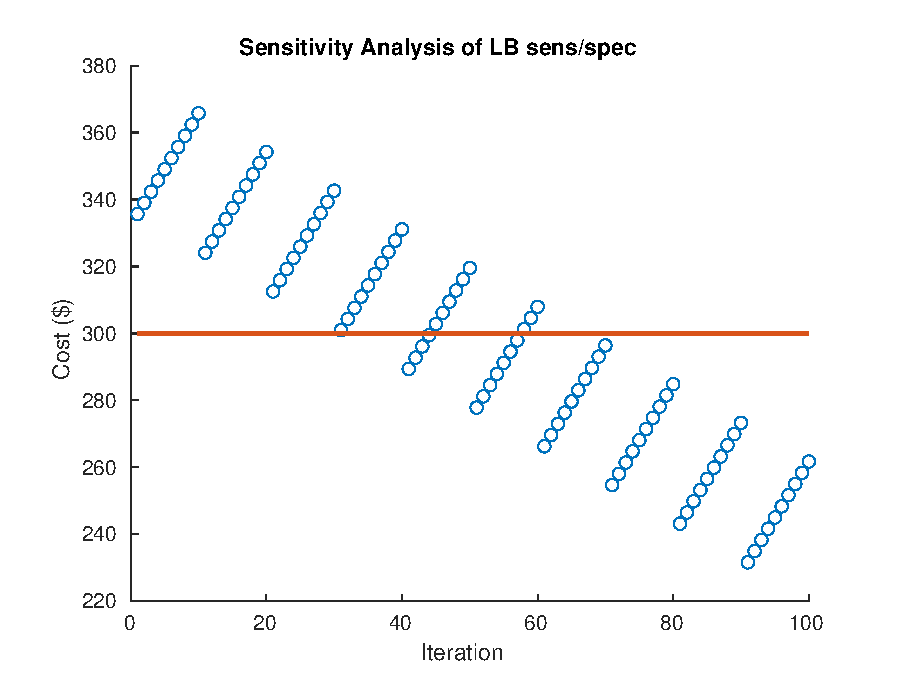
\includegraphics[width = .49\textwidth]{3d_2}

\textit{\underline{49\%} of the simulated outputs for cost difference were greater than 300.}

\end{frame}

\begin{frame}[fragile]
\frametitle{Sample-Based Sensitivity Analysis}
Here is a verification that my sampling was done correctly. I created a brute-force method for orthogonal sampling, \verb|orth_samples.m|. 

\vspace{1em}
\centering
\hspace*{-2cm}                                                           
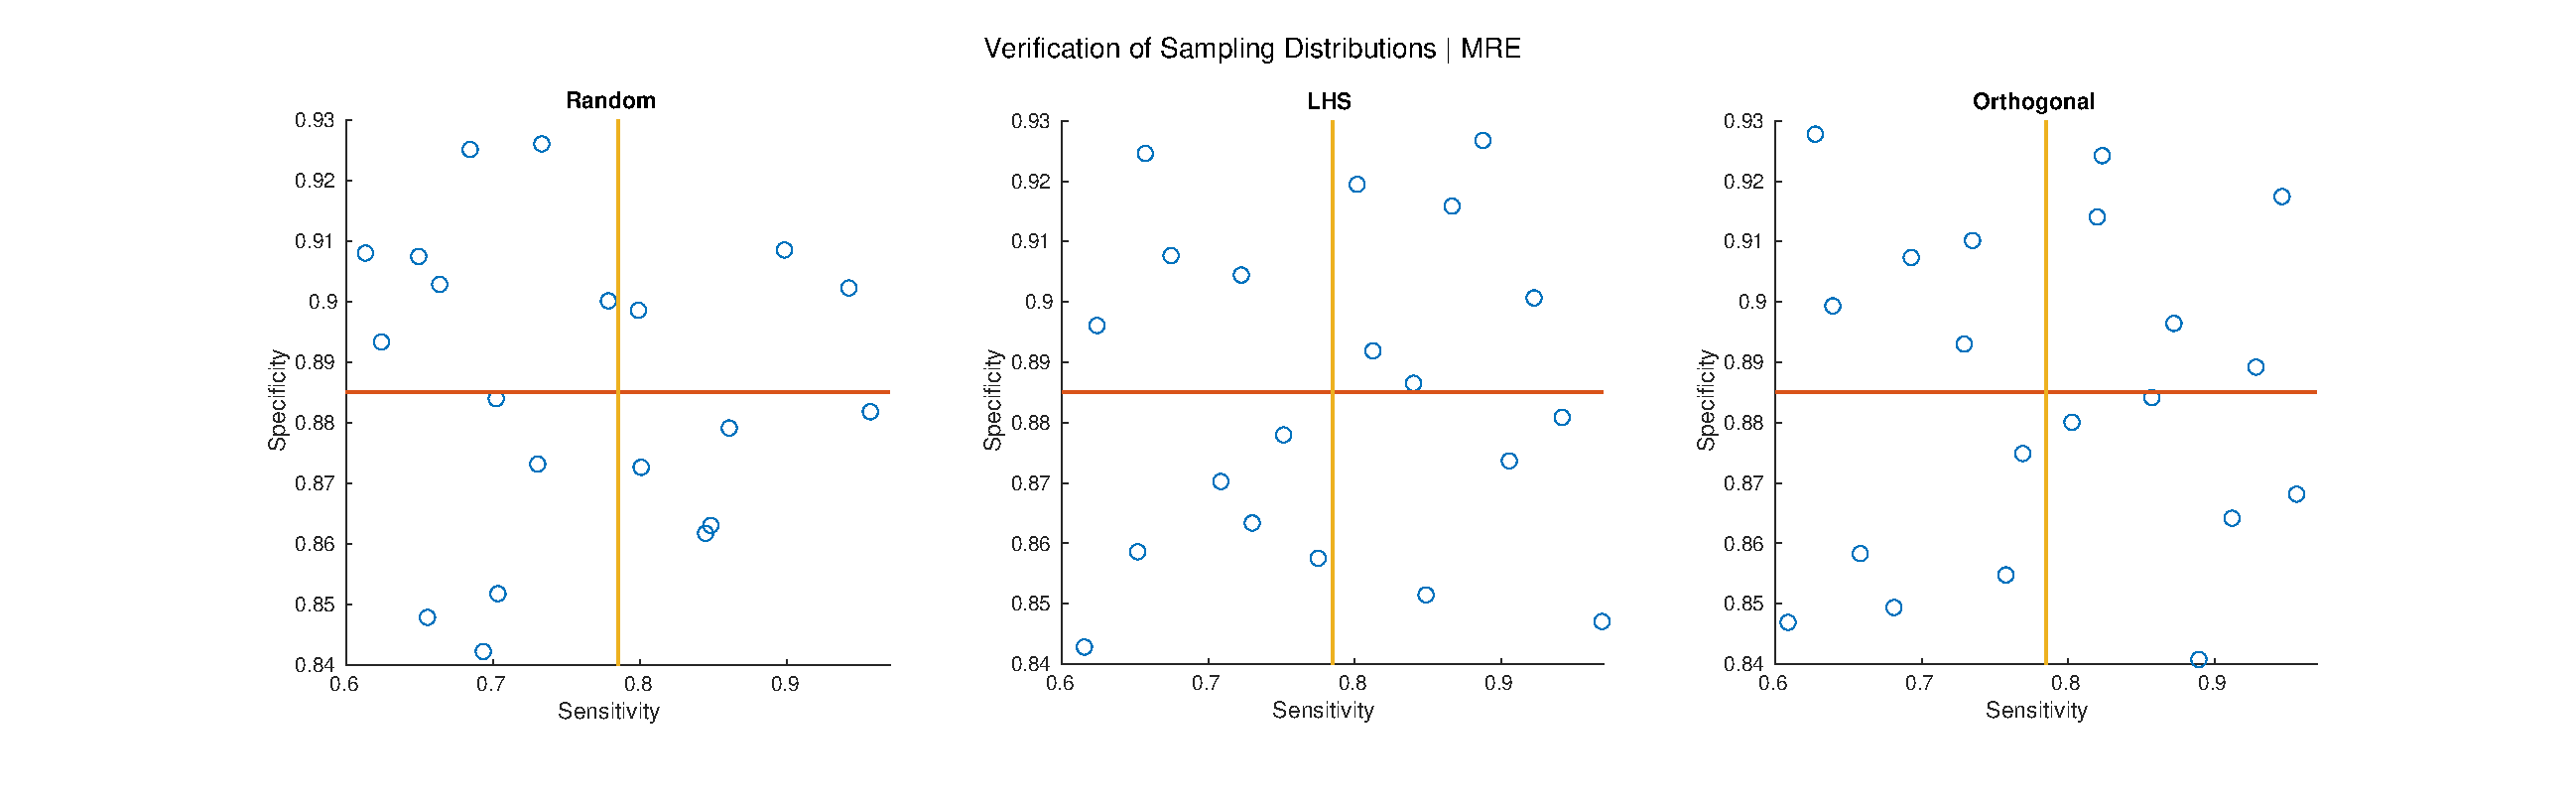
\includegraphics[scale = .41]{sampling_ex}
\end{frame}

\begin{frame}
\frametitle{Question 3e $|$ Sample-Based Sensitivity Analysis for \underline{MRE}}
Here are the 3D plots, regression equations and Pearson's correlation coefficients for the MRE sample-based Sensitivity Analysis. 

\vspace{1em}
\centering                                                         
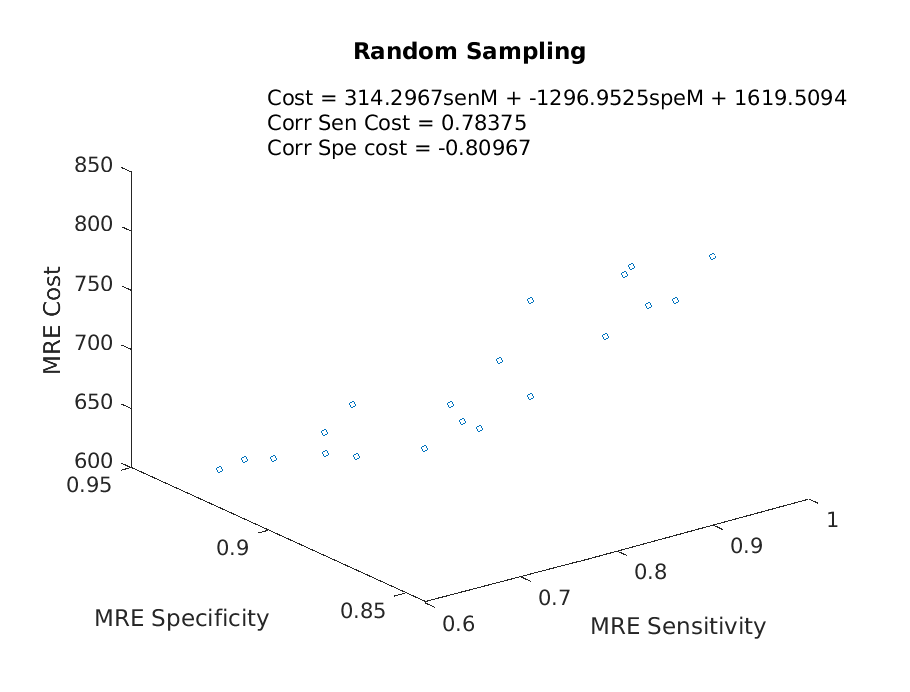
\includegraphics[scale = .3]{mre1}
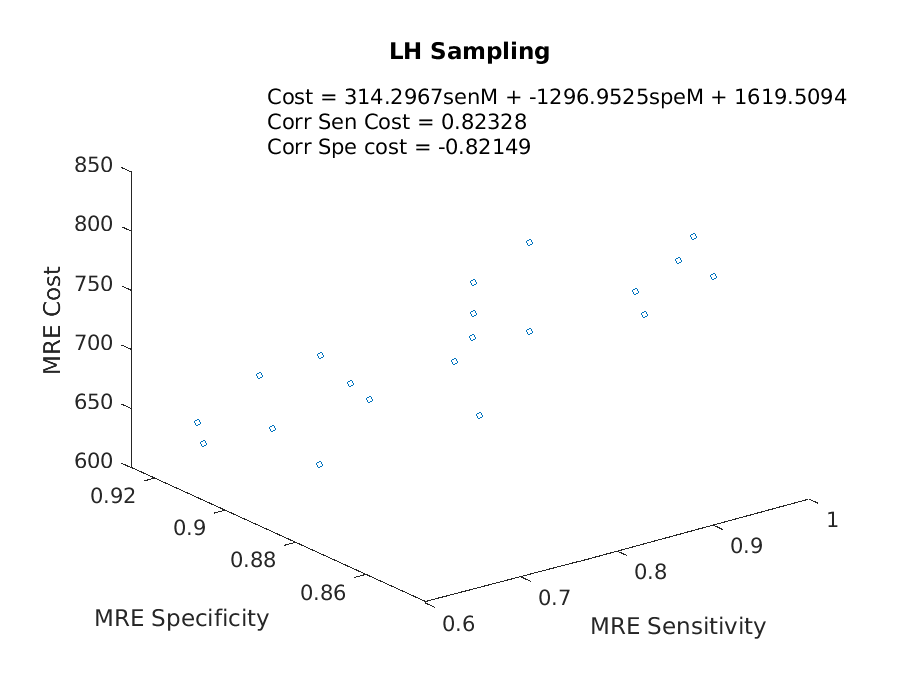
\includegraphics[scale = .3]{mre2}
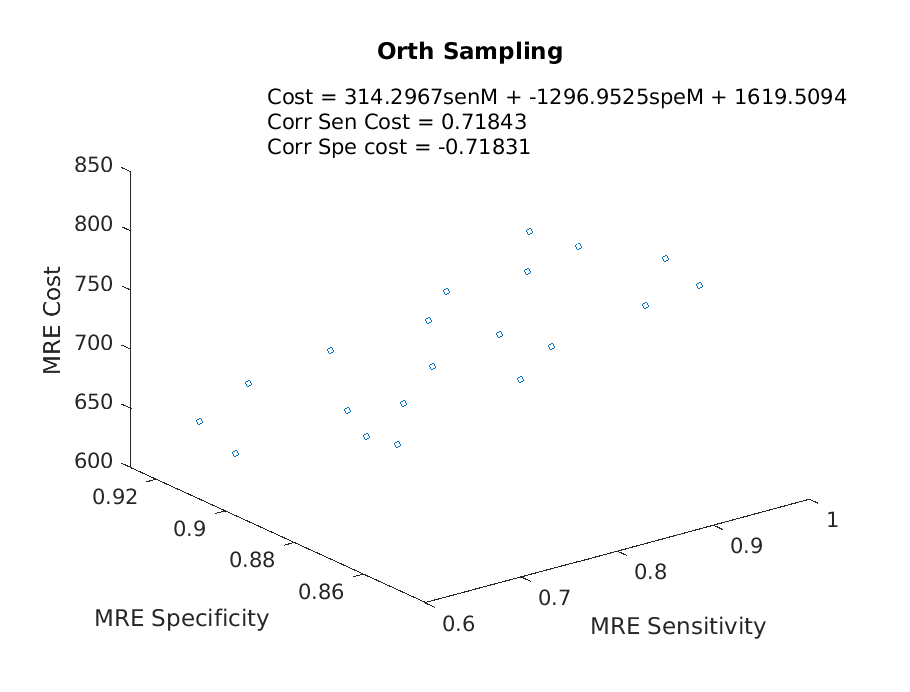
\includegraphics[scale = .3]{mre3}\\
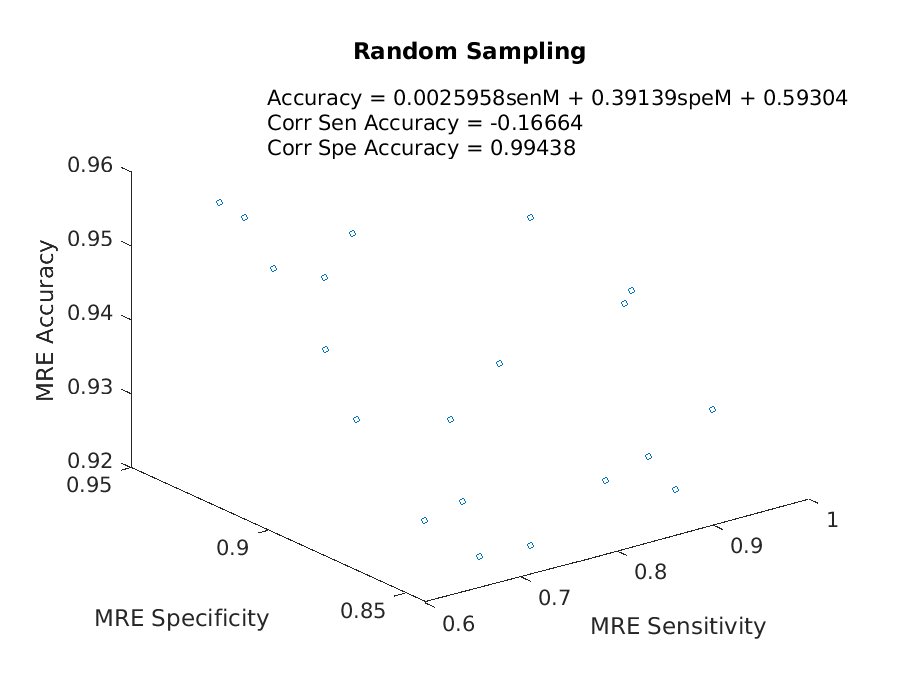
\includegraphics[scale = .3]{mre4}
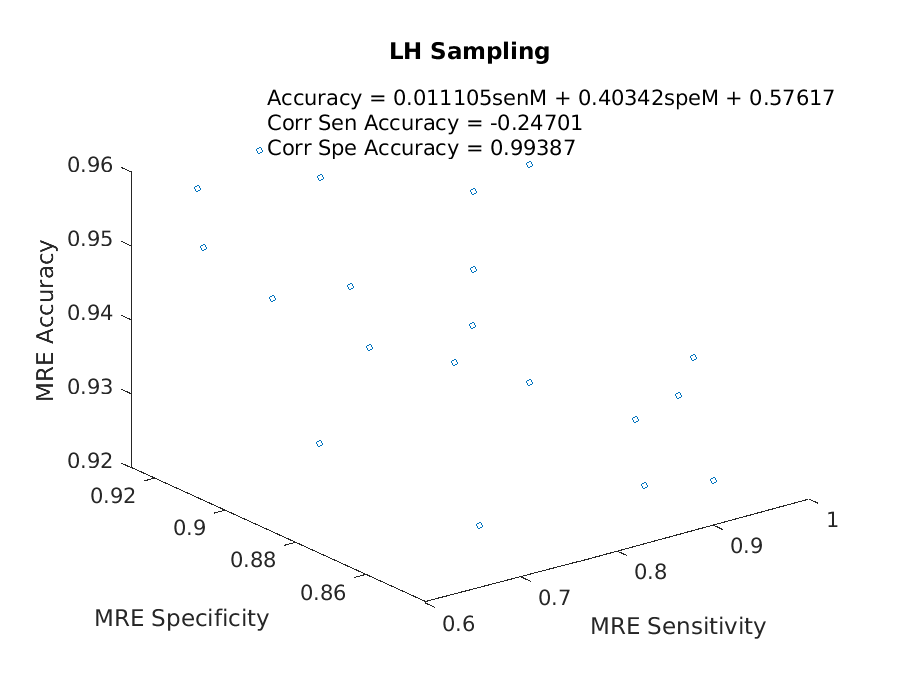
\includegraphics[scale = .3]{mre5}
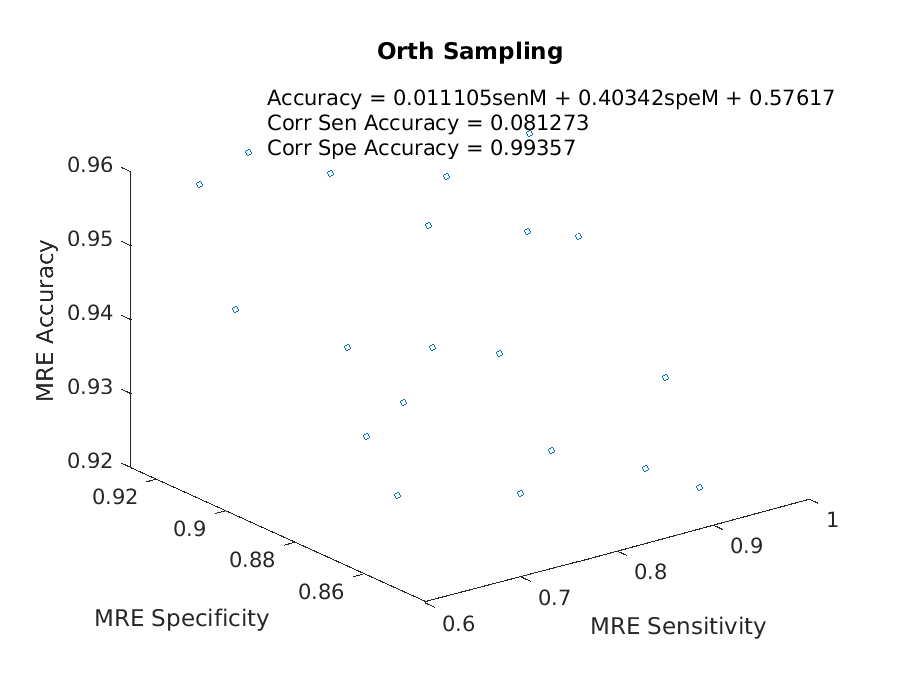
\includegraphics[scale = .3]{mre6}
\end{frame}

\begin{frame}
\frametitle{Question 3f $|$ Sample-Based Sensitivity Analysis for \underline{LB}}
Here are the 3D plots, regression equations and Pearson's correlation coefficients for the LB sample-based Sensitivity Analysis. 

\vspace{1em}
\centering                                                         
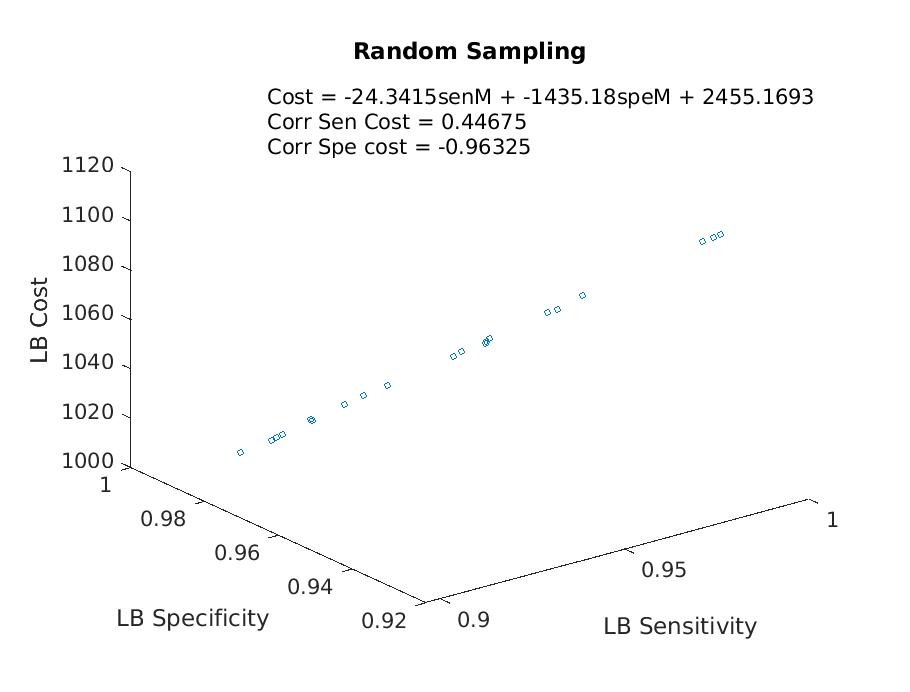
\includegraphics[scale = .3]{lb1}
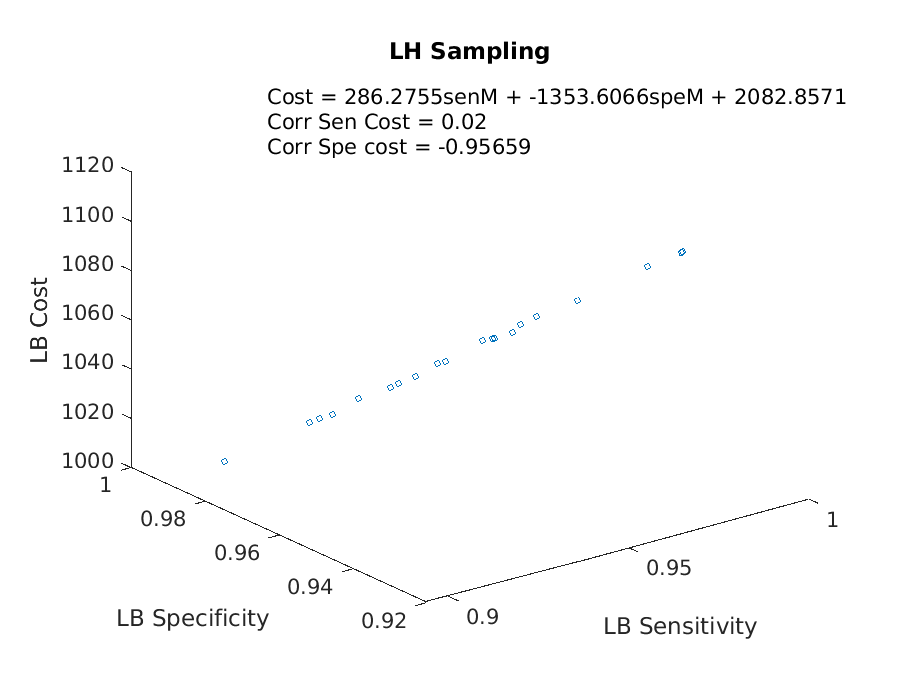
\includegraphics[scale = .3]{lb2}
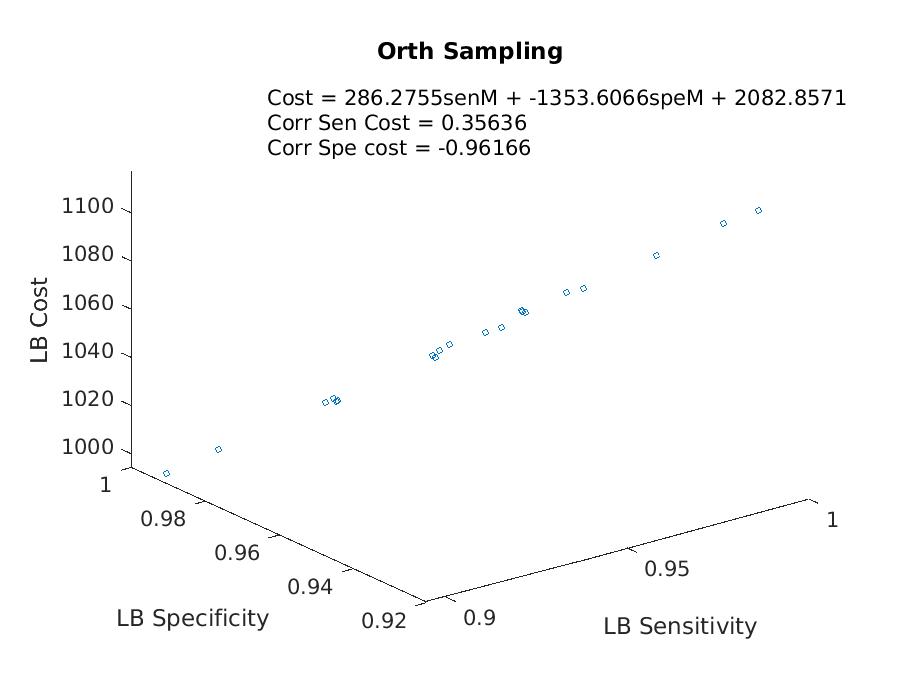
\includegraphics[scale = .3]{lb3}\\
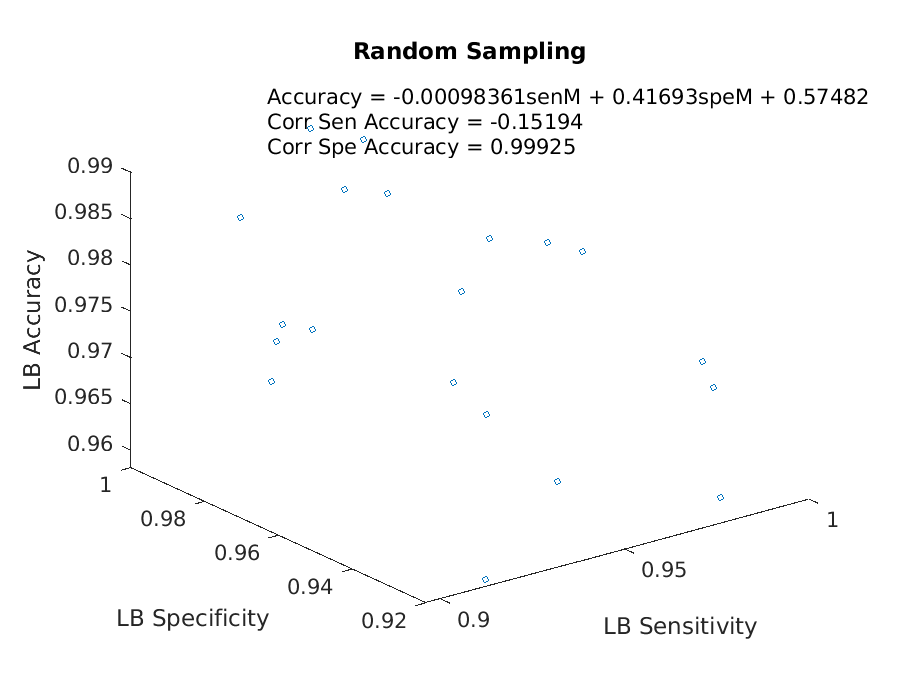
\includegraphics[scale = .3]{lb4}
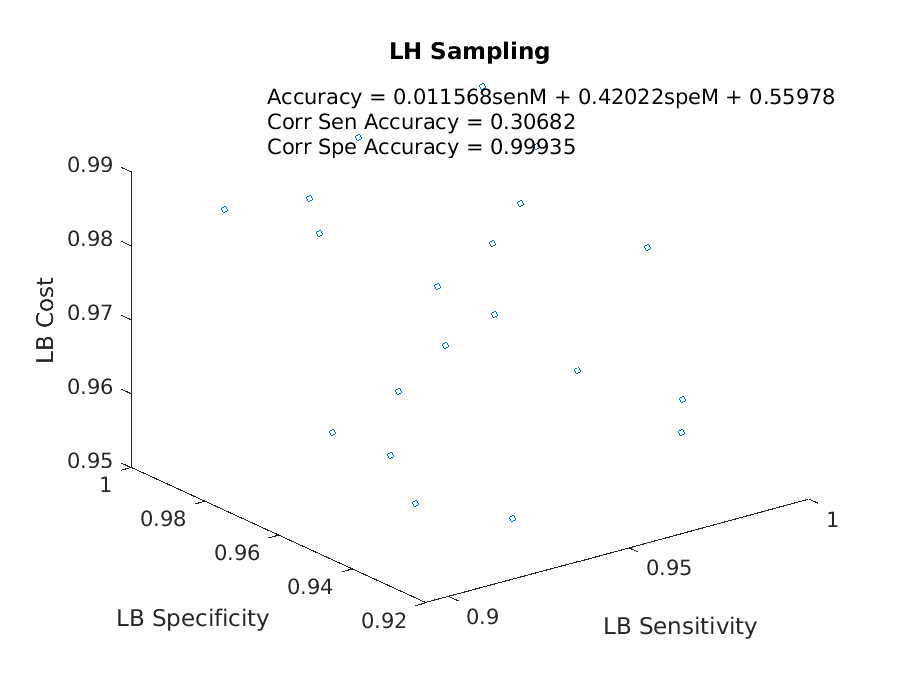
\includegraphics[scale = .3]{lb5}
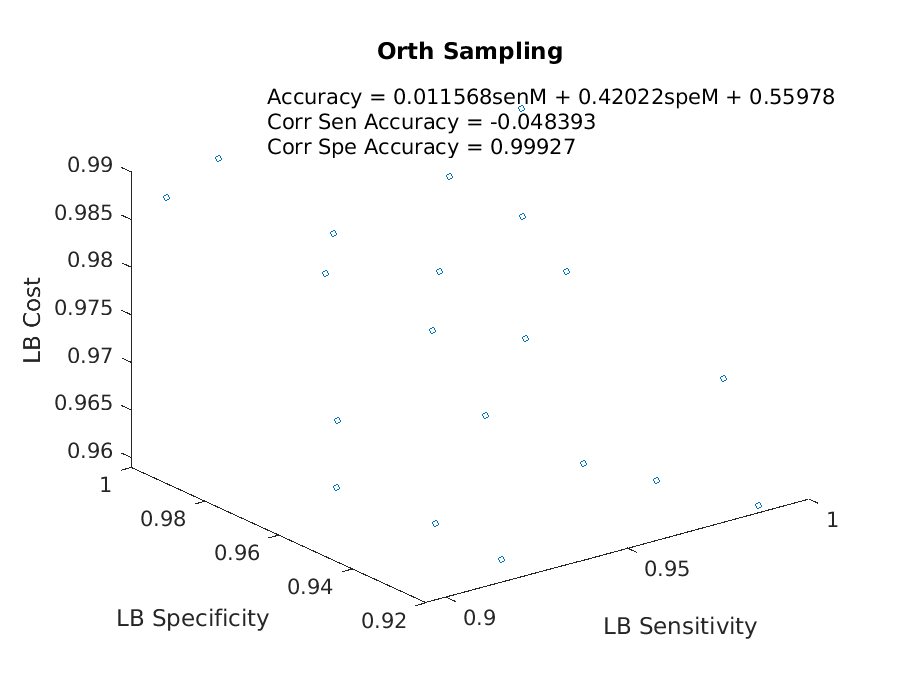
\includegraphics[scale = .3]{lb6}
\end{frame}


\end{document}